\documentclass{article}
\usepackage{tikz}
\title{TikZ Practice}
\author{Federico Revoltella}
\date{January 2026}

\begin{document}

\maketitle

\section{Introduction}

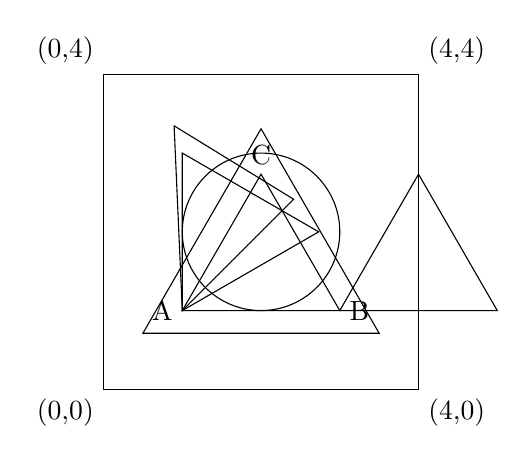
\begin{tikzpicture}


% Part A: Shapes


% Square
\draw (0,0)--(4,0)--(4,4)--(0,4)--cycle;

% Circle
\draw (2,2) circle (1);

% Triangle ABC
\draw (1,1)-- (3,1) - - (2,2.732)-  - cycle;


% Part B: Labels


% Square labels
\node[below left]  at (0,0) {(0,0)} ;
\node[below right] at (4,0) {(4,0)}  ;
\node[above right] at (4,4) {(4,4)};
\node[above left]  at (0,4) {(0,4) } ;

% Triangle labels
\node[left]  at (1,1) {A};
\node[right] at (3,1) {B};
\node[above] at (2,2.732) {C};

% Part C: Translation (+2, 0)

\draw (3,1)--(5,1)--(4,2.732)--cycle;


% Part C: Reflection over y=x

\draw (1,1)--(1,3)--(2.732,2)- -cycle;


% Part D: Scaling (1.5x about centroid)
% Centroid ≈ (2, 1.577)

\draw (0.5,0.712)--(3.5,0.712)--(2,3.309)--cycle;


% Part D: Rotation (45° about A)

\draw (1,1)--(2.414,2.414)--(0.896,3.346)--cycle;

\end{tikzpicture}
\end{document}
